\documentclass[journal,12pt,twocolumn]{IEEEtran}
\usepackage{setspace}
\usepackage{gensymb}
\usepackage{caption}
%\usepackage{multirow}
%\usepackage{multicolumn}
%\usepackage{subcaption}
%\doublespacing
\singlespacing
\usepackage{csvsimple}
\usepackage{amsmath}
\usepackage{multicol}
%\usepackage{enumerate}
\usepackage{amssymb}
%\usepackage{graphicx}
\usepackage{newfloat}
%\usepackage{syntax}
\usepackage{listings}
\usepackage{iithtlc}
\usepackage{color}
\usepackage{tikz}
\usetikzlibrary{shapes,arrows}



%\usepackage{graphicx}
%\usepackage{amssymb}
%\usepackage{relsize}
%\usepackage[cmex10]{amsmath}
%\usepackage{mathtools}
%\usepackage{amsthm}
%\interdisplaylinepenalty=2500
%\savesymbol{iint}
%\usepackage{txfonts}
%\restoresymbol{TXF}{iint}
%\usepackage{wasysym}
\usepackage{amsthm}
\usepackage{mathrsfs}
\usepackage{txfonts}
\usepackage{stfloats}
\usepackage{cite}
\usepackage{cases}
\usepackage{mathtools}
\usepackage{caption}
\usepackage{enumerate}	
\usepackage{enumitem}
\usepackage{amsmath}
%\usepackage{xtab}
\usepackage{longtable}
\usepackage{multirow}
%\usepackage{algorithm}
%\usepackage{algpseudocode}
\usepackage{enumitem}
\usepackage{mathtools}
\usepackage{hyperref}
%\usepackage[framemethod=tikz]{mdframed}
\usepackage{listings}
    %\usepackage[latin1]{inputenc}                                 %%
    \usepackage{color}                                            %%
    \usepackage{array}                                            %%
    \usepackage{longtable}                                        %%
    \usepackage{calc}                                             %%
    \usepackage{multirow}                                         %%
    \usepackage{hhline}                                           %%
    \usepackage{ifthen}                                           %%
  %optionally (for landscape tables embedded in another document): %%
    \usepackage{lscape}     


\usepackage{url}
\def\UrlBreaks{\do\/\do-}


%\usepackage{stmaryrd}


%\usepackage{wasysym}
%\newcounter{MYtempeqncnt}
\DeclareMathOperator*{\Res}{Res}
%\renewcommand{\baselinestretch}{2}
\renewcommand\thesection{\arabic{section}}
\renewcommand\thesubsection{\thesection.\arabic{subsection}}
\renewcommand\thesubsubsection{\thesubsection.\arabic{subsubsection}}

\renewcommand\thesectiondis{\arabic{section}}
\renewcommand\thesubsectiondis{\thesectiondis.\arabic{subsection}}
\renewcommand\thesubsubsectiondis{\thesubsectiondis.\arabic{subsubsection}}

% correct bad hyphenation here
\hyphenation{op-tical net-works semi-conduc-tor}

%\lstset{
%language=C,
%frame=single, 
%breaklines=true
%}

%\lstset{
	%%basicstyle=\small\ttfamily\bfseries,
	%%numberstyle=\small\ttfamily,
	%language=Octave,
	%backgroundcolor=\color{white},
	%%frame=single,
	%%keywordstyle=\bfseries,
	%%breaklines=true,
	%%showstringspaces=false,
	%%xleftmargin=-10mm,
	%%aboveskip=-1mm,
	%%belowskip=0mm
%}

%\surroundwithmdframed[width=\columnwidth]{lstlisting}
\def\inputGnumericTable{}                                 %%
\lstset{
%language=C,
frame=single, 
breaklines=true,
columns=fullflexible
}
 

\begin{document}
%
\tikzstyle{block} = [rectangle, draw,
    text width=3em, text centered, minimum height=3em]
\tikzstyle{sum} = [draw, circle, node distance=3cm]
\tikzstyle{input} = [coordinate]
\tikzstyle{output} = [coordinate]
\tikzstyle{pinstyle} = [pin edge={to-,thin,black}]

\theoremstyle{definition}
\newtheorem{theorem}{Theorem}[section]
\newtheorem{problem}{Problem}
\newtheorem{proposition}{Proposition}[section]
\newtheorem{lemma}{Lemma}[section]
\newtheorem{corollary}[theorem]{Corollary}
\newtheorem{example}{Example}[section]
\newtheorem{definition}{Definition}[section]
%\newtheorem{algorithm}{Algorithm}[section]
%\newtheorem{cor}{Corollary}
\newcommand{\BEQA}{\begin{eqnarray}}
\newcommand{\EEQA}{\end{eqnarray}}
\newcommand{\define}{\stackrel{\triangle}{=}}

\bibliographystyle{IEEEtran}
%\bibliographystyle{ieeetr}

\providecommand{\nCr}[2]{\,^{#1}C_{#2}} % nCr
\providecommand{\nPr}[2]{\,^{#1}P_{#2}} % nPr
\providecommand{\mbf}{\mathbf}
\providecommand{\pr}[1]{\ensuremath{\Pr\left(#1\right)}}
\providecommand{\qfunc}[1]{\ensuremath{Q\left(#1\right)}}
\providecommand{\sbrak}[1]{\ensuremath{{}\left[#1\right]}}
\providecommand{\lsbrak}[1]{\ensuremath{{}\left[#1\right.}}
\providecommand{\rsbrak}[1]{\ensuremath{{}\left.#1\right]}}
\providecommand{\brak}[1]{\ensuremath{\left(#1\right)}}
\providecommand{\lbrak}[1]{\ensuremath{\left(#1\right.}}
\providecommand{\rbrak}[1]{\ensuremath{\left.#1\right)}}
\providecommand{\cbrak}[1]{\ensuremath{\left\{#1\right\}}}
\providecommand{\lcbrak}[1]{\ensuremath{\left\{#1\right.}}
\providecommand{\rcbrak}[1]{\ensuremath{\left.#1\right\}}}
\theoremstyle{remark}
\newtheorem{rem}{Remark}
\newcommand{\sgn}{\mathop{\mathrm{sgn}}}
\providecommand{\abs}[1]{\left\vert#1\right\vert}
\providecommand{\res}[1]{\Res\displaylimits_{#1}} 
\providecommand{\norm}[1]{\lVert#1\rVert}
\providecommand{\mtx}[1]{\mathbf{#1}}
\providecommand{\mean}[1]{E\left[ #1 \right]}
\providecommand{\fourier}{\overset{\mathcal{F}}{ \rightleftharpoons}}
%\providecommand{\hilbert}{\overset{\mathcal{H}}{ \rightleftharpoons}}
\providecommand{\system}{\overset{\mathcal{H}}{ \longleftrightarrow}}
	%\newcommand{\solution}[2]{\textbf{Solution:}{#1}}
\newcommand{\solution}{\noindent \textbf{Solution: }}
\newcommand{\myvec}[1]{\ensuremath{\begin{pmatrix}#1\end{pmatrix}}}
\providecommand{\dec}[2]{\ensuremath{\overset{#1}{\underset{#2}{\gtrless}}}}
\DeclarePairedDelimiter{\ceil}{\lceil}{\rceil}
%\numberwithin{equation}{section}
%\numberwithin{problem}{subsection}
%\numberwithin{definition}{subsection}
\makeatletter
\@addtoreset{figure}{section}
\makeatother

\let\StandardTheFigure\thefigure
%\renewcommand{\thefigure}{\theproblem.\arabic{figure}}
\renewcommand{\thefigure}{\thesection}


%\numberwithin{figure}{subsection}

%\numberwithin{equation}{subsection}
%\numberwithin{equation}{section}
%\numberwithin{equation}{problem}
%\numberwithin{problem}{subsection}
\numberwithin{problem}{section}
%%\numberwithin{definition}{subsection}
%\makeatletter
%\@addtoreset{figure}{problem}
%\makeatother
\makeatletter
\@addtoreset{table}{section}
\makeatother

\let\StandardTheFigure\thefigure
\let\StandardTheTable\thetable
\let\vec\mathbf
%%\renewcommand{\thefigure}{\theproblem.\arabic{figure}}
%\renewcommand{\thefigure}{\theproblem}

%%\numberwithin{figure}{section}

%%\numberwithin{figure}{subsection}



\def\putbox#1#2#3{\makebox[0in][l]{\makebox[#1][l]{}\raisebox{\baselineskip}[0in][0in]{\raisebox{#2}[0in][0in]{#3}}}}
     \def\rightbox#1{\makebox[0in][r]{#1}}
     \def\centbox#1{\makebox[0in]{#1}}
     \def\topbox#1{\raisebox{-\baselineskip}[0in][0in]{#1}}
     \def\midbox#1{\raisebox{-0.5\baselineskip}[0in][0in]{#1}}

\vspace{3cm}

\title{ 
	\logo{
The Straight Line and Linearity
	}
}

\author{ G V V Sharma$^{*}$% <-this % stops a space
	\thanks{*The author is with the Department
		of Electrical Engineering, Indian Institute of Technology, Hyderabad
		502285 India e-mail:  gadepall@iith.ac.in. All content in this manual is released under GNU GPL.  Free and open source.}
	
}	

\maketitle

%\tableofcontents

\bigskip

\renewcommand{\thefigure}{\theenumi}
\renewcommand{\thetable}{\theenumi}


\begin{abstract}
	Solved problems from JEE mains papers related to 2D lines in coordinate geometry are 
available in this document.  These problems are solved using linear algebra/matrix analysis.
\end{abstract}
\begin{enumerate}[label=\arabic*]
\numberwithin{equation}{enumi}

\item A straight line through the origin   $\vec{O}$ meets the lines
\begin{align} 
\label{eq:line_1}
\myvec{4 & 3}\vec{x} &= 10
\\
\myvec{8 & 6}\vec{x} +5&= 0
\end{align} 
%
at $\vec{A}$ and $\vec{B}$ respectively.  Find the ratio in which  $\vec{O}$ divides $AB$.
\\
\solution Let 
\begin{align} 
\vec{n} =\myvec{4 \\ 3}
\end{align} 
%
Then \eqref{eq:line_1} can be expressed as
\begin{align} 
\label{eq:line_1_normal}
\vec{n}^T\vec{x} &= 10
\\
2\vec{n}^T\vec{x} &= -5
\end{align} 
%
and since $\vec{A}, \vec{B}$ satisfy \eqref{eq:line_1_normal} respectively,
\begin{align} 
\label{eq:line_1_normal_a}
\vec{n}^T\vec{A} &= 10
\\
2\vec{n}^T\vec{B} &= -5
\label{eq:line_1_normal_b}
\end{align} 
%
Let  $\vec{O}$ divide the segment $AB$ in the ratio $k:1$. Then
\begin{align} 
\label{eq:line_1_section}
\vec{O}=\frac{k\vec{B} +\vec{A} }{k+1}
\end{align} 
%
\begin{align} 
%\label{eq:line_1_section}
\because \vec{O}&= \vec{0},
\\
\vec{A} &=-k\vec{B}
\end{align} 
%
Substituting in \eqref{eq:line_1_normal_a}, and simplifying, 
\begin{align} 
\label{eq:line_1_normal_subs_a}
\vec{n}^T\vec{B} &= \frac{10}{-k}
\\
\vec{n}^T\vec{B} &= \frac{-5}{2}
%\label{eq:line_1_normal_b}
\end{align} 
resulting in 
\begin{align} 
\frac{10}{-k} = \frac{-5}{2} \implies k = 4
\end{align} 
\item The 
point 
\begin{equation} 
\vec{P}=\myvec{2\\ 1} 
\end{equation} 
is translated parallel to the line 
\begin{equation} 
\label{line_2}
L: \myvec{1 & -1}\vec{x} = 4 
\end{equation} 
% 
by $d =2\sqrt{3}$ units.  If the new point $\vec{Q}$ lies in the third 
quadrant, then find the equation of the line passing through $\vec{Q}$ and perpendicular to $L$. 
\\
\solution From \eqref{line_2}, the direction vector of $L$ is
\begin{equation} 
\label{line_2_m}
\vec{m} = \myvec{1 \\ 1} 
\end{equation} 
Thus, 
\begin{equation} 
\label{line_2_q}
\vec{Q}= \vec{P} + \lambda \vec{m}
\end{equation} 
However, 
\begin{align} 
PQ &= d
\\
\implies\norm{\vec{P}- \vec{Q}} &= \abs{\lambda}\norm{\vec{m}} =  d
\\
\implies \lambda &= \pm \frac{d}{\norm{\vec{m}}} = \pm \sqrt{6}
\label{line_2_lam}
\end{align} 
%
\begin{align} 
\because \norm{\vec{m}} = \sqrt{\vec{m}^T\vec{m}}= \sqrt{2}
\end{align} 
%
from \eqref{line_2_m}.  Since $\vec{Q}$ lies in the third quadrant, from \eqref{line_2_q} and \eqref{line_2_lam},
\begin{align} 
\vec{Q} = \myvec{2\\ 1}  -  \sqrt{6}\myvec{1\\ 1} =  \myvec{2-\sqrt{6}\\ 1-\sqrt{6}}
\end{align} 
%
The equation of the desired line is then obtained as 
\begin{align} 
\label{line_2_final}
\vec{m}^T\brak{\vec{x}-\vec{Q}}&= 0
\\
 \myvec{1 & 1}\vec{x} &= 3 -2\sqrt{6}
\end{align} 
\item Two sides of a rhombus are along the lines
\begin{align}
\label{eq:lines_4_ab}
AB: \myvec{1 & -1}\vec{x} + 1 &=0
\\
AD: \myvec{7 & -1}\vec{x} -5 &=0.
\label{eq:lines_4_ad}
\end{align}
%
If its diagonals intersect at 
\begin{equation}
\vec{P}=\myvec{-1\\ -2},
\label{eq:lines_4_p}
\end{equation}
find its vertices.
\\
\solution From \eqref{eq:lines_4_ab} and \eqref{eq:lines_4_ad},
\begin{align}
\myvec{1 & -1 \\ 7 & -1}\vec{A}  &=\myvec{-1 \\ 5}
\end{align}
%
By row reducing the augmented matrix
\begin{align}
\myvec{1 & -1 & -1\\ 7 & -1 & 5}  &\leftrightarrow \myvec{1 & -1 & -1\\ 0 & 6 & 12}\leftrightarrow \myvec{1 & -1 & -1\\ 0 & 1 & 2}
\nonumber \\
&\leftrightarrow \myvec{1 & 0 & 1\\ 0 & 1 & 2} \implies \vec{A}=\myvec{1\\ 2},
\label{eq:lines_4_a}
\end{align}
%
Since diagonals of a rhombus bisect each other, 
\begin{align}
\vec{P}&=\frac{\vec{A}+\vec{C}}{2}
\nonumber \\
\vec{C}&=2\vec{P}-\vec{A} = \myvec{-3\\-6}
\label{eq:lines_4_c}
\end{align}
%
\begin{align}
\because AD \parallel BC,&
\nonumber \\
BC: \myvec{7 & -1}\brak{\vec{x}-\vec{C}} &=0
\nonumber \\
\implies \myvec{7 & -1}\vec{x} &=-15
\label{eq:lines_4_bc}
\end{align}
%
From \eqref{eq:lines_4_ab} and \eqref{eq:lines_4_bc},
\begin{align}
 \myvec{7 & -1 \\ 1 & -1}\vec{B} &=\myvec{-15 \\ -1}
\end{align}
resulting in the augmented matrix
\begin{align}
& \myvec{7 & -1 & -15\\ 1 & -1 & -1} 
\leftrightarrow
 \myvec{7 & -1 & -15\\ 0 & 3 & -4} 
\nonumber \\
&\leftrightarrow
 \myvec{3 & 0 & -7\\ 0 & 3 & -4} \implies \vec{B} = -\frac{1}{3}\myvec{7\\4}
\end{align}
\begin{align}
\because AB \parallel CD,&
\nonumber \\
CD: \myvec{1 & -1}\brak{\vec{x}-\vec{C}} &=0
\nonumber \\
\implies \myvec{1 & -1}\vec{x} &=3
\label{eq:lines_4_cd}
\end{align}
%
From \eqref{eq:lines_4_ad} and \eqref{eq:lines_4_cd},
\begin{align}
 \myvec{7 & -1 \\ 1 & -1}\vec{D} &=\myvec{5 \\ 3}
\end{align}
resulting in the augmented matrix
\begin{align}
& \myvec{7 & -1 & 5\\ 1 & -1 & 3} 
\leftrightarrow
 \myvec{7 & -1 & 5\\ 0 & 3 & -8} 
\nonumber \\
&\leftrightarrow
 \myvec{3 & 0 & 1\\ 0 & 3 & -8} \implies \vec{D} = \frac{1}{3}\myvec{1\\-8}
\end{align}

%From \eqref{eq:lines_4_p} and \eqref{eq:lines_4_a}
%\begin{align}
%AP =\norm{\vec{A}-\vec{P}} = 2\sqrt{5} =d (say)
%\end{align}
%%
%The direction vector of $AP$ is 
%\begin{align}
%\vec{m} &=\vec{A}-\vec{P} = 2\myvec{1\\ 2}
%\\
%\implies \norm{\vec{m}} &= 2\sqrt{5}
%\end{align}
%Since the direction of $AP$ is the same as $AC$,
%\begin{align}
%\vec{C} &=\vec{P}-d\frac{\vec{m}}{\norm{\vec{m}}} 
%\nonumber \\
%&= -\myvec{1\\ 2}- 2\myvec{1\\ 2} = \myvec{-3\\ -6}
%\end{align}
%
%Let $\vec{n}\perp\vec{m}$. Then 
%\begin{align}
%\vec{n} &=\myvec{2\\ -1}
%\end{align}
%%
%and 
%\begin{align}
%\vec{B,D} &=\vec{P}\pm d\frac{\vec{n}}{\norm{\vec{n}}} 
%\nonumber \\
%&=-\myvec{1\\ 2}\pm 2\myvec{2\\ -1} = \myvec{5\\ 0}, \myvec{-3\\ 4}
%\end{align}

\item Let $k$ be an integer such that the triangle with vertices
\begin{equation}
\label{eq:lines_5}
\vec{A} = \myvec{k\\-3k},
\vec{B} =\myvec{5\\k},
\vec{C} =\myvec{-k\\2}
\end{equation}
has area 28.  Find the orthocentre of this triangle.
%
\\
\solution Let $\vec{m}_1$ be the direction vector of $BC$.  Then,
\begin{align}
\label{eq:lines_5_m1}
\vec{m}_1 = \myvec{5+k\\k-2},
\end{align}
%
If $AD$ be an altitude, its equation can be obtained as
\begin{align}
\label{eq:lines_5_m1a}
\vec{m}_1^{T}\brak{\vec{x}-\vec{A}} = 0
\end{align}
%
Similarly, considering the side $AC$  the equation of the altitude $BE$ is
\begin{align}
\label{eq:lines_5_m2b}
\vec{m}_2^{T}\brak{\vec{x}-\vec{B}} = 0
\end{align}
%
where 
\begin{align}
\label{eq:lines_5_m2}
\vec{m}_2 = \myvec{2k\\-2-3k},
\end{align}
The orthocentre is obtained by solving \eqref{eq:lines_5_m1a}
and \eqref{eq:lines_5_m2b} using the matrix equation
\begin{align}
\myvec{\vec{m}_1\\ \vec{m}_2}^T \vec{x} 
= \myvec{ \vec{m}_1^T\vec{A}\\ \vec{m}_2^T
\vec{B}}
\end{align}
%
which can be expressed using \eqref{eq:lines_5_m1}, 
\eqref{eq:lines_5_m2}, 
\eqref{eq:lines_5_m1a} and 
\eqref{eq:lines_5_m2b}
as 
\begin{align}
\myvec{5+k & k-2 \\2k & -2-3k} \vec{x} 
&= \myvec{ k^2+5k+6k-3k^2\\ 10k-2k-3k^2}
\nonumber \\
&= k\myvec{ 11-4k\\ 8-3k}
\label{eq:lines_5_h}
\end{align}
%
%The solution to the above is 
%\begin{align}
%\vec{x} &= k\myvec{5+k & k-2 \\2k & -2-3k}^{-1} \myvec{ 11-4k\\ 8-3k}
%\nonumber \\
%&= \frac{k}{-3k^2-17k-10-2k^2+4k}
%\nonumber \\
%&\times \myvec{-2-3k & -k+2 \\-2k & 5+k} \myvec{ 11-4k\\ 8-3k}
%\nonumber \\
%&= \frac{k}{5k^2+13k+10}
%\nonumber \\
%&\times \myvec{2+3k & k-2 \\2k & -5-k} \myvec{ 11-4k\\ 8-3k}
%\nonumber \\
%&= \frac{k}{5k^2+13k+10}
%\nonumber \\
%&\times 
%\myvec{ 22-12k^2-8k+33k -3k^2+6k+8k-16 \\ 22k-8k^2-40+15k-8k+3k^2}
%\nonumber \\
%&= \frac{k}{5k^2+13k+10}
%\myvec{ 6+39k-15k^2 \\ -40+29k-5k^2}
%\end{align}
From \eqref{eq:lines_5}, using the expression for the area of triangle,
\begin{align}
\begin{vmatrix}
k & 5 & -k\\-3k & k & 2 \\ 1 & 1 & 1
\end{vmatrix} = 56
\nonumber \\
\implies
\begin{vmatrix}
k & 5-k & -2k\\-3k & 4k & 2+3k \\ 1 & 0 & 0
\end{vmatrix} = 56
\end{align}
%
resulting in
\begin{align}
\brak{5-k}
\brak{2+3k}+8k^2=56
\\
\implies 5k^2+13k-46 = 0
\\
\text{or, } k = 2, -\frac{23}{5}
\end{align}
Substituting the above in \eqref{eq:lines_5_h} and solving yields the orthocentre.
\item If an equilateral triangle, having centroid at the origin, has a side along the line
\begin{equation}
\label{eq:lines_6_ab}
\myvec{1 & 1}\vec{x} = 2,
\end{equation}
then find the area of this triangle. Also draw the equilateral triangle and two medians to verify your results.
\\
\solution Let the vertices be $\vec{A},\vec{B},\vec{C}$. From the given information, 
\begin{align}
\frac{\vec{A}+\vec{B}+\vec{C}}{3} &= \vec{0}
\nonumber \\
\implies 
\vec{A}+\vec{B}+\vec{C} = \vec{0}
\label{eq:lines_6_abc}
\end{align}
%
If $AB$ be the line in \eqref{eq:lines_6_ab},
%\begin{equation}
%\label{eq:lines_6_nab}
%\myvec{1 & 1}\brak{\vec{A}-\vec{B}} = 0
%\end{equation}
%%
%Thus, the direction vector of $AB$ is 
%\begin{align}
%\label{eq:lines_6_mab}
%\vec{m} = \myvec{1 \\ -1}
%\end{align}
the equation of 
$CF$, where 
\begin{align}
\vec{F} = \frac{\vec{A}+\vec{B}}{2} 
\end{align}
is 
%
\begin{align}
\label{eq:lines_6_cf}
\myvec{1 & -1}\vec{x} = 0
\end{align}
since $CF$ passes through the origin and $CF\perp AB$. From \eqref{eq:lines_6_ab}
and \eqref{eq:lines_6_cf},
\begin{align}
\label{eq:lines_6_fmat}
\myvec{1 & 1 \\1 & -1}\vec{F} = \myvec{2 \\ 0}
\end{align}
%
Forming the augmented matrix, 
\begin{align}
\myvec{1 & 1 &2 \\1 & -1 & 0} &\leftrightarrow \myvec{1 & 1 &2 \\0 & 2 & 2} \leftrightarrow \myvec{1 & 1 &2 \\0 & 1 & 1} 
\nonumber \\
&\leftrightarrow \myvec{1 & 0 &1 \\0 & 1 & 1} \implies \vec{F} = \myvec{1 \\ 1}
\label{eq:lines_6_f}
\end{align}
From \eqref{eq:lines_6_abc},
\begin{align}
\vec{C}=-\brak{\vec{A}+\vec{B}}=-2\vec{F} = -2\myvec{1 \\ 1}
\label{eq:lines_6_c}
\end{align}
after substituting from \eqref{eq:lines_6_f}.  Thus, 
\begin{align}
CF &= \norm{\vec{C}-\vec{F}} = 3\sqrt{2} 
\\
\implies AB &=  CF\frac{2}{\sqrt{3}} = 2\sqrt{6}
\label{eq:lines_6_cflen}
\end{align}
and the area of the triangle is 
\begin{align}
\frac{1}{2} AB \times CF = 6\sqrt{3}
\end{align}


\item A square, of each side 2, lies above the $x$-axis and has one vertex at the origin.  If one of the sides 
passing through the origin makes an angle $30^{\degree}$ with the positive direction of the $x$-axis, then 
find the 
sum of the $x$-coordinates of the vertices of the square.
\\
\solution Consider the square $ABCD$ with $\vec{A} = \vec{0}, AB = 2$ such that $\vec{B}$ and $\vec{D}$ lie on the $x$ and $y$-axis respectively. Then 
\begin{align}
\vec{A}+\vec{B}+\vec{C}+\vec{D} = 4\myvec{1 \\ 1}
\label{eq:lines_7_abcdsum}
\end{align}
%
Multiplying \eqref{eq:lines_7_abcdsum} with the rotation matrix 
\begin{align}
\label{eq:lines_7_t}
\vec{T} = \myvec{\cos \theta & -\sin \theta \\ \sin \theta & \cos \theta},
\end{align}
\begin{align}
\vec{T}\brak{\vec{A}+\vec{B}+\vec{C}+\vec{D}} &= 4\myvec{\cos \theta & -\sin \theta \\ \sin \theta & \cos \theta}\myvec{1 \\ 1}
\nonumber \\
&= 4\myvec{\cos \theta  -\sin \theta \\ \cos \theta + \sin \theta}
%\nonumber \\
\end{align}
\begin{multline}
\implies \myvec{1 & 0}\vec{T}\brak{\vec{A}+\vec{B}+\vec{C}+\vec{D}} 
\\
= 4\brak{\cos \theta  -\sin \theta}
= 2\brak{\sqrt{3}-1}
\end{multline}
%
for $\theta = 30^{\degree}$. Draw the square with sides on the axis as well as the rotated square in the same graph to verify your result.


%\item Find the locus of the point of intersection of the lines
%\begin{align}
%\myvec{\sqrt{2} & -1 }\vec{x} + 4 \sqrt{2}k &= 0
%\\
%\myvec{\sqrt{2}k & k }\vec{x} - 4 \sqrt{2} &= 0
%\end{align}

\end{enumerate}
\section{Trigonometry}
\begin{enumerate}[label=\thesection.\arabic*
,ref=\thesection.\theenumi]

\item In $\triangle PQR$, which is not right angled, let
\begin{align}
PQ = r, QR = p, RP = q
\end{align}
%
The median $RS$ and the altitude $PE$  intersect at $\vec{O}$. $p =\sqrt{3}, q = 1$ and the radius of the circumcircle  of $\triangle PQR = k = 1$.  
\item Find  $RS$
\\
\solution Using the sine formula,
\begin{align}
\frac{p}{\sin P}=\frac{q}{\sin Q} = 2k
\\
\implies \sin P = \frac{\sqrt{3}}{2}, \sin Q = \frac{1}{2}
\end{align}
If $\angle R \ne \frac{\pi}{2}$, the only possible solution is 
\begin{align}
\angle P = \frac{2\pi}{3},
\angle Q = \frac{\pi}{6},
\angle R = \frac{\pi}{6}
\end{align}
%
$\because \angle Q = \angle R, q = r = 1$.  The given information is shown in Fig. \ref{fig:2019_8}
\begin{figure}
\centering
\includegraphics[width=\columnwidth]{./figs/2019_8.eps}
\caption{}
\label{fig:2019_8}
\end{figure}
%
Using the cosine formula, 
\begin{align}
RS &= \sqrt{q^2+\brak{\frac{r}{2}}^2-qr\cos P}
\\
&= \sqrt{1+\frac{1}{4}+\frac{1}{2}} = \sqrt{\frac{7}{2}}
\end{align}
\item Find $OE$.
\\
\solution 
Using Baudhayana's theorem,
\begin{align}
OE  &= \sqrt{OR^2 - ER^2}
\\
&= \sqrt{\brak{\frac{2RS}{3}}^2 - \brak{\frac{p}{2}}^2} 
\\
&= \sqrt{\frac{7}{9}-\frac{3}{4}} = \frac{1 }{6}
\end{align}
%
\item Find the area of $\triangle SOE$
\\
\solution
$\because$ $PE$ and $RS$ are medians, 
\begin{align}
\text{ar}\brak{\triangle SOE }&= \frac{1}{4}\text{ar}\brak{\triangle POR},
\\
\text{ar}\brak{\triangle POR }&=  \frac{2}{3}\text{ar}\brak{\triangle PER},
\\
\text{ar}\brak{\triangle PER }&=  \frac{1}{2}\text{ar}\brak{\triangle PQR},
\\
\implies \text{ar}\brak{\triangle SOE} &= \frac{1}{12}\text{ar}\brak{\triangle PQR}
&= \frac{\sqrt{3}}{24}
\end{align}

\item Find the radius of the incircle of $\triangle PQR $.
%
\\
\solution
I is the incentre in Fig. \ref{fig:2019_8}.  The radius of the incircle is 
\begin{align}
\frac{p}{2\cos\frac{Q}{2}} &= \frac{p}{\sqrt{2\brak{1+\cos Q}}}
\\ &= \sqrt{\frac{3}{1+\sqrt{3}}}
\end{align}
%
\item Repeat all the above exercises using vector algebra and plot Fig. \ref{fig:2019_8}.
\end{enumerate}
%
\end{document}
